

 
  \documentclass[11pt]{article}

\usepackage{amsmath,amssymb}
    \usepackage{url}
\thispagestyle{empty}
\usepackage[all]{xy}
\SelectTips{cm}{}
\usepackage{tikz}
\usetikzlibrary{arrows,shapes,snakes,automata,backgrounds,petri,patterns}
\usepackage{pxfonts}
\oddsidemargin 0pt
\evensidemargin 0 pt
\topmargin -.3in
\headsep 20pt
\footskip 20pt
\textheight 8.5in
\textwidth 6.25in
\newcommand{\modelsall}[1]{\models{\mkern-15mu}\raise5pt\hbox{$\scriptstyle#1$}}

 \newcommand{\forces}{\,\mbox{$\mathrel\|\mathrel{\mkern-9mu}-\,$}}
\renewcommand{\ni}{\noindent}
\newcommand{\hearts}{\textcolor{red}{\varheartsuit}}
\newcommand{\diamonds}{\textcolor{red}{\vardiamondsuit}}
\newcommand{\clubs}{\clubsuit}
\newcommand{\Kbar}{\overline{K}}
\newcommand{\Fin}{\mbox{Fin}}
\newcommand{\Tot}{\mbox{Tot}}
\newcommand{\Inf}{\mbox{Inf}}
\newcommand{\Con}{\mbox{Con}}
\newcommand{\Cof}{\mbox{Cof}}
\newcommand{\Cput}{\mbox{Cput}}
\newcommand{\Ext}{\mbox{Ext}}
\newcommand{\dar}{\!\downarrow}
\newcommand{\uar}{\!\uparrow}
\newcommand{\A}{\cal A}
\def\aext#1{\widetilde{#1}}
\newcommand{\adamek}{Ad\'{a}mek}
\renewcommand{\phi}{\varphi}
\newcommand{\fv}[1]{{\mathsf{fv}}(#1)}
\let\maps\colon  
\newcommand{\mng}[1]{[\!\![ #1 ]\!\!]} 
\newcommand{\rem}[1]{\relax}
\newcommand{\afa}{\mbox{\it AFA}}
\newcommand{\fc}[1]{\overline{#1}}
\newcommand{\fcalt}[1]{{\widehat{#1}}}
\newcommand{\abar}{\fc{a}}
\newcommand{\bbar}{\fc{b}}
\newcommand{\cbar}{\fc{c}}
\newcommand{\abaralt}{\fcalt{a}}
\newcommand{\bbaralt}{\fcalt{b}}
\newcommand{\cbaralt}{\fcalt{c}}
\newcommand{\nbar}{\fc{n}}
\newcommand{\mbar}{\fc{m}}
\newcommand{\pbar}{\fc{p}}
\newcommand{\nbaralt}{\fcalt{n}}
\newcommand{\mbaralt}{\fcalt{m}}
\newcommand{\pbaralt}{\fcalt{p}}
\newcommand{\sbar}{\fc{s}}
\newcommand{\fbar}{\fc{f}}
\newcommand{\gbar}{\fc{g}}
\newcommand{\ubar}{\fc{u}}
\newcommand{\Vbar}{\fc{V}}
\newcommand{\Vbarbar}{\overline{\overline{V}}}
\newcommand{\abarbar}{\overline{\overline{a}}}
\newcommand{\bbarbar}{\overline{\overline{b}}}
\newcommand{\vbar}{\vvec}
\newcommand{\AFA}{\mbox{\it AFA}}
%%%\newcommand{\id}{{\it id}}
\newcommand{\Set}{{\catfont{Set}}}
\newcommand{\Sets}{{\catfont{Class}}}
\newcommand{\Class}{{\catfont{Class}}}
\newcommand{\Sat}{{\it Sat}}
\newcommand{\AtProp}{{\sf AtProp}}
\newcommand{\bisim}{\equiv}
\newcommand{\nec}{\Box}
\newcommand{\necc}{\Box}
\newcommand{\pos}{\lozenge}
\newcommand{\poss}{\lozenge}
\newcommand{\fr}{\it{Fr}}
\newcommand{\strex}{\it{StrEx}}
\newcommand{\Pow}{{\cal P}}
\newcommand{\dagalt}{\uparrow}
\newcommand{\iif}{\rightarrow}
\newcommand{\iiff}{\leftrightarrow}
\newcommand{\sbstut}[2]{[#2]#1} 

\newcommand{\lang}{{\cal L}}
\newcommand{\mang}{{\cal M}}

\def\T#1{\mathcal{T}(#1)}
\renewcommand{\L}{{T}^{\Pow}}

\newcommand{\Gfinal}{\overline{\G}}

\newcommand{\D}{\Delta}
\newcommand{\functorf}{{\sf F}}
\newcommand{\set}[1]{\{#1\}}
\newcommand{\functorI}{{\sf I}}
\newcommand{\sem}[1]{[\![ #1{]\!]}}
\newcommand{\pair}[1]{\langle #1\rangle}
\newcommand{\pairalt}[1]{\langle#1\rangle}
\newcommand{\EE}{{\cal E}}
\renewcommand{\AA}{{\cal A}}
\newcommand{\K}{K}
\newcommand{\KB}{KB}
\newcommand{\Kfour}{K4}
\newcommand{\Sfour}{S4}
\newcommand{\Sfive}{S5}
\newcommand{\FF}{{\cal F}}
\newcommand{\RR}{{\cal R}}
\newcommand{\UU}{{\cal U}}
\newcommand{\id}{{\sf id}}
\newcommand{\incl}{i}
\newcommand{\inl}{{\sf inl}}
\newcommand{\inr}{{\sf inr}}
\newcommand{\nat}{{\sf nat}}
\newcommand{\ch}{{\sf ch}}
\newcommand{\emphterm}[1]{{\em #1}}
\newcommand{\fmla}[2]{\forall #1(#2)}
\newcommand{\st}{\mbox{\rm $\kern .3em%
|\kern -.25em | \kern -.25em | \kern .4em$}}
\newcommand{\identical}{\equiv}
\newcommand{\quadidentical}{\quad \identical \quad}
\newcommand{\Image}{{\it Image}}
\newcommand{\restr}{\,{\upharpoonleft}\,}
\newcommand{\inflang}{{\cal L}}
\newcommand{\overlinej}{{k}}
\newcommand{\proves}{\vdash}
\newcommand{\Proves}{\mbox{\it Proves}}
\renewcommand{\Pr}{\mbox{\it Pr}}
\newcommand{\pow}{{\cal P}}
\newcommand{\powfin}{{\cal P}_{\scriptstyle{fin}}}
\newcommand{\quadeq}{\quad = \quad}
\newcommand{\quadequiv}{\quad \equiv \quad}
\newcommand{\quadiff}{\quad \mbox{iff} \quad}
\newcommand{\quadsubseteq}{\quad \subseteq \quad}
\newcommand{\first}{\mbox{$\pi_1$}}
%\newcommand{\first}{\mbox{$1^{\it st}$}}
\newcommand{\map}[3]{#1\,:#2 \rightarrow #3}
\newcommand{\inclusionmap}[3]{#1\,:#2 \hookrightarrow #3}
%\newcommand{\second}{\mbox{$2^{\it nd}$}}
\newcommand{\langp}{{\cal M}}
\newcommand{\ntrans}[3]{#1\,: #2 \rightarrow #3}
\newcommand{\second}{\mbox{$\pi_2$}}
\newcommand{\true}{\top}
\newcommand{\false}{\bot}
\newcommand{\andd}{\wedge}
\newcommand{\orr}{\vee}
\newcommand{\On}{\mbox{\it On}}
\newcommand{\nott}{\neg}
\newcommand{\tri}{\triangle}
\newcommand{\Vafa}{V_{\it afa}}
\newcommand{\sfnew}{{\sf new}}
\newcommand{\supp}[1]{{\it support}#1}
\newcommand{\dom}{{\it dom}}
\newcommand{\ZFM}{\mbox{{\it ZFC}$^-$}}
\newcommand{\ZFA}{\mbox{\it ZFA}}
\newcommand{\ZFC}{\mbox{\it ZFC}}
\newcommand{\zfc}{\ZFC}
\newcommand{\Zfc}{\ZFC}
\newcommand{\zf}{\mbox{\it ZF}}
\newcommand{\Vwf}{V_{{\it wf}}}
\newcommand{\FA}{FA}
\newcommand{\FinSeq}{\mbox{\it FinSeq}}
\newcommand{\ProbG}{{\sf P}}
\renewcommand{\t}{\true}
\newtheorem{exer}{Exercise}
\renewcommand{\circ}{\o}
\renewcommand{\H}{H}
%\newcommand{\T}{T}
\newcommand{\flro}{\mbox{{\it FLR}$_0$}}
\newcommand{\flri}{\mbox{{\it FLR}$_1$}}
\newcommand{\flr}{\flri}
\newcommand{\val}{\Lambda}
\newcommand{\abovearrow}[1]{\rightarrow\hspace{-.17in}\raisebox{1.0ex}
{$\scriptscriptstyle{#1}$}\hspace{.1in}}
\newcommand{\arrowa}{\,\lower1pt\hbox{$\abovearrow{a}$}}
\newcommand{\arrowb}{\,\lower1pt\hbox{$\abovearrow{b}$}}

\newcommand{\casedef}{\left\{\begin{array}{ll}}
\newcommand{\bekic}{Beki\v{c}}
\newcommand{\Bekic}{\bekic}
\newcommand{\card}[1]{|#1|}
\renewcommand{\dag}{\dagger}
\newcommand{\valof}[3]{\val_{#1}(#2)\,#3}
\newcommand{\where}[2]{\,#1\ {\tt where}\ \{#2\}\,}
\newcommand{\whereleftonly}[2]{\,#1\ {\tt where}\ \{#2 \,}
\newcommand{\whererightonly}[1]{\,#1\ \}\,}

%\newcommand{\textbf}[1]{\mbox{\bf #1}}
%\newcommand{\textrm}[1]{\mbox{\rm #1}}
%\newcommand{\mathrm}[1]{\mbox{\rm #1}}
%\newcommand{\mathsf}[1]{\mbox{\sf #1}}

\newcommand{\row}[2]{{#1}_{#1},\ldots, {#1}_{#2}}\newcommand{\vv}[1]{\mbox{\sf #1}}
\renewcommand{\o}{\cdot}
\def\sol#1{{#1}^{\dag}}
%\def\funsol{\sol{(\,\_\,)}}
\newcommand{\wbar}{\overline{w}}
\newcommand{\xvec}{\overline{x}}
\newcommand{\xbar}{\xvec}%% since I always mess these up
\newcommand{\ybar}{\yvec}
\newcommand{\zbar}{\zvec}
\newcommand{\pixvec}{\vec{\pi x}}
\newcommand{\pixhat}{\pixvec}
\newcommand{\Val}{\val}
\newcommand{\SD}{\sf SD}
\newcommand{\CC}{{\cal S}}
\newcommand{\partto}{\rightharpoonup}
 \newcommand{\recw}[2]{\mbox{\bf rec}(#1)\{#2\}} %alternate for where
\newcommand{\heart}{\heartsuit}
\newcommand{\club}{\clubsuit}
\renewcommand{\diamond}{\diamondsuit}
\newcommand{\spade}{\spadesuit}
\newcommand{\one}{\mbox{\tt 1}}
\newcommand{\monus} {-\hspace{-.125in}\raisebox{1.0ex}
{$\scriptstyle{\bullet}$}\hspace{.1in}}
\newcommand{\hash}{\mbox{\tt \#}}

\newcommand{\provesH}{\vdash_{\!\!\!  \lower2pt\hbox{$\scriptstyle \sf H$}}}
\newcommand{\provesSfive}{\vdash_{\!\!\!  \lower2pt\hbox{$\scriptstyle \sf S5$}}}
\newcommand{\provesSfiveH}{\vdash_{\!\!\!  \lower2pt\hbox{$\scriptstyle \sf S5-H$}}}
\newcommand{\modelseq}{\models_{\!\!\!  \lower2pt\hbox{$\scriptstyle \sf eq$}}}

 \newcommand{\seat}{\mid\hspace{-.04in}\raisebox{-1.74ex}{$\rightsquare$}}
\def\rightsqr#1#2#3#4{{\mathclose{\kern-.#4em\raise#3ex\vbox{\hrule
    height.#2pt\hbox{\kern#1ex \vrule width.#2pt
    height #1ex}}\hbox{\hskip.2em}}}}
\def\leftsquare{\leftsqr{.7}2{1.15}{1}}
\def\rightsquare{\rightsqr{.7}2{1.15}{1}}\begin{document}
 
 
\begin{center}
{
\Large  Modal Logic, Winter 2019   \\
Homework 10\\
Due Tuesday,  April 9 \\
}
\end{center}
\newcommand{\heads}{h}
\newcommand{\tails}{t}
\newcommand{\Heads}{h}
\newcommand{\Tails}{t}
\newcommand{\Model}{{\cal M}}
\newcommand{\Nodel}{{\cal N}}
\newcommand{\Pub}{\relax}
\begin{enumerate}

 \item
 Here is a model which we've seen before
 
$$
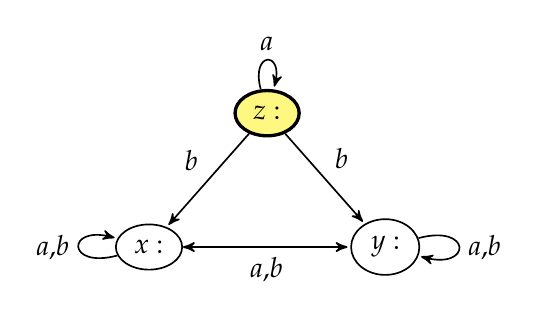
\begin{tikzpicture}[<->,>=stealth',shorten >=1pt,auto,node distance=4cm,semithick]
\tikzstyle{every ellipse node}= [draw]
\path (-1.5,0) node[ellipse]  (x) {$x: \Heads $}  --
 (1.5,0) node[ellipse,draw](y)  {$y: \Tails$} ;
 \path (0,1.7) node[ellipse,fill=yellow!50,very thick] (z) {$z: \Heads $};
 %\path[<->] (x) edge  (y);
\draw (x) -- (y) [swap] node[midway,below]   {$a$,$b$};
% \draw[<->]  (x) -- {$a$,$b$} (y);
\path[->] (x) edge [loop left]  node {$a$,$b$} (x);
\path[->] (y) edge [loop right] node {$a$,$b$} (y);
\path[->] (z) edge [loop above] node {$a$} (z);
\path[->](z) edge node[swap]  {$b$} (x);
\path[->](z) edge node {$b$} (y);
 \end{tikzpicture}
 $$
\begin{enumerate}
\item True or false:  $z \forces CK_{a,b} \nott K_b\ K_a \ h$, where $h$ is ``heads.''
\item True or false:  $z \forces CK_{a,b} K_b\nott  K_a \ h$, where $h$ is ``heads.''
\end{enumerate}

 

\item Recall that throughout our semester, letters like $p$ denote
\emph{atomic sentences}.    Show that $\models_{all} [p]CK_{\cal A} \, p$.
Here ${\cal A}$ is the set of all agents.   Intuitively, 
$[p]CK_{\cal A}\, p$ says, ``if $p$ is true, then announcing it truthfully to everyone
results in $p$ becoming common knowledge.''
\label{ck}

\vfil\eject

\item Recall the coin scenarios from our worksheet:
\paragraph{Scenario 0}
Two people, \emph{Amina (A)} (female) and \emph{Bao (B)} (male), enter a large room.
On the table, is   
 a remote-control mechanical coin flipper.
 One presses a button, and the coin spins through the
air, landing 
in a small box on the table. 
The box closes.
  The two people are much too far
to see the coin.
In  {reality}, the coin shows heads.

\paragraph{Scenario 2}
After Scenario 0, $A$ goes up and looks at the coin while $B$ stands at the door.
$B$ watches her open the box, but he doesn't see what she sees.


We symbolize the situation after Scenario 2 by
$$
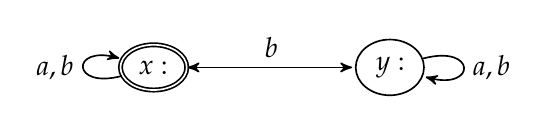
\begin{tikzpicture}[<->,>=stealth',shorten >=1pt,auto,node distance=4cm,semithick]
\tikzstyle{every ellipse node}= [draw]
\path (-1.5,0) node[ellipse,double]  (x) {$x: \Heads $}  --
 (1.5,0) node[ellipse,draw](y)  {$y: \Tails$} ;
%\path[<->] (x) edge  (y);
\draw (x) -- (y) node[midway,above] {$b$};
% \draw[<->]  (x) -- {a,b} (y);
\path[->] (x) edge [loop left]  node {$a,b$} (x);
\path[->] (y) edge [loop right] node {$a,b$} (y);
 \end{tikzpicture}
 $$
Now consider the following sentences:
 $$\begin{array}{lcl}
 \phi_{ht} &  &  \Heads\oplus\Tails = (\Heads\orr\Tails) \andd\nott (\Heads\andd\Tails) \\
  \phi^*&  & ((\heads\andd K_a \heads \andd P_a \heads)\orr (\tails \andd K_a \tails \andd P_a \tails))
   \andd\ \nott K_b\, \heads\
 \andd \ \nott K_b\, \tails\\

 \psi & & \phi_{ht} \andd \phi^* \andd CK_{a,b}(\phi_{ht}\andd\phi^*)  \\
 \chi_{\Heads} & & \Heads \andd \psi \\
 \chi_{\Tails} & & \Tails \andd \psi \\
 \end{array}
 $$
 Here, $P\phi$ is the ``$\diamond$ version of $K$''.
 That is, $P_a\Heads$ is an abbreviation of $\nott K_a \nott\Heads$.
 And for all $z$, $z\models P_a\Heads$ if there is some $w$ such that $z\arrowa w$ and $w\models\Heads$.
 
 

 Let $\Nodel$ be any model of $\chi_h$, \emph{not necessarily the model shown above}.
Your job is to show that all of the following hold about satisfaction in $\Nodel$:
 \begin{enumerate}
\item 
  If $w\models \chi_{\Heads}$, then there is some $v$ such that $w\arrowa v$ 
and $v\models  \chi_{\Heads}$.

\item   If $w\models \chi_{\Heads}$, then every $v$ such that $w\arrowa v$  
has $v\models  \chi_{\Heads}$.


\item 
  If $w\models \chi_{\tails}$, then there is some $v$ such that $w\arrowa v$ 
and $v\models  \chi_{\Tails}$.

\item  If $w\models \chi_{\tails}$,  then every $v$ such that $w\arrowa v$  
has $v\models  \chi_{\tails}$.




\item 
  If $w\models \chi_{\Heads}$, then there is some $v$ such that $w\arrowb v$ 
and $v\models  \chi_{\Heads}$.


\item 
  If $w\models \chi_{\Heads}$, then there is some $v$ such that $w\arrowb v$ 
and $v\models  \chi_{\Tails}$.


\item  If $w\models \chi_{\Heads}$,  then every $v$ such that $w\arrowa v$  
has $v\models  \chi_{\Heads}$ or $v\models  \chi_{\Tails}$.


\item 
  If $w\models \chi_{\Tails}$, then there is some $v$ such that $w\arrowb v$ 
and $v\models  \chi_{\Heads}$.


\item 
  If $w\models \chi_{\Tails}$, then there is some $v$ such that $w\arrowb v$ 
and $v\models  \chi_{\Tails}$.


\item   If $w\models \chi_{\Tails}$, then every $v$ such that $w\arrowb v$  
has $v\models  \chi_{\Heads}$ or $v\models  \chi_{\Tails}$.




\end{enumerate}

[Hint: All of the parts are fairly short semantic arguments (a few sentences each), 
and the key steps
involve the use of the Mix Axiom. 
You also can say that some parts are similar to others.   For example,
(f), (i), and (h) are all similar to (e); you can say this.
Similarly, (j) is similar to (g).]
 

\item  (The knowledge flip-flop)
 Suppose we have four players: Amina, Bao,  Chandra, and Dianne.
They have a deck with two indistinguishable $\spadesuit$
cards, one $\diamondsuit$ and one $\clubsuit$.
  The cards are dealt, and the players look at their own cards.
  
  We assume that the
following are common knowledge:  the distribution of cards in   the
deck, the fact that each player   knows which card was dealt to
them, and that they do not initially know any other player's card.

 

The deal is
$$  w \quadeq (A\spadesuit,B\spadesuit,C\diamondsuit,D\clubsuit).$$
So this is the ``real world'', and we call this world $w$.

We take a modal language with atomic sentences
$$A\spadesuit, A\diamondsuit, A\clubsuit, 
B\spadesuit, B\diamondsuit, B\clubsuit,
C\spadesuit, C\diamondsuit, C\clubsuit,
D\spadesuit, D\diamondsuit, D\clubsuit,
$$
We have agents $a$, $b$, $c$, and $d$, and so we have knowledge sentences 
involving those agents.  We shall be concerned with the sentence $\phi$, given as
$$\nott K_b \, A\spadesuit \ \andd\ \nott K_b \, A\diamondsuit\ \andd\
\nott K_b \, A\clubsuit.$$
It says that Bao doesn't know Amina's that Amina has spaces, he also doesn't know that she has diamonds,
and in addition he doesn't know that Amina has clubs.


\begin{enumerate}
\item  Show that  $w\forces K_c\, \phi$.

\item  Then Amina announces, ``I do not have $\diamondsuit$.''
Show that now $w\forces \nott K_c\, \phi$.

\item After this,  Dianne announces, ``I do not have $\spadesuit$.''
Show that now  $w\forces K_c\, \phi$.

\end{enumerate}
You \emph{can} solve this problem by constructing the initial model explictly.
It has twelve worlds.    Some people will no doubt prefer to do this, since it is very concrete
and also satisfying.    But you don't \emph{have} to do it this way.   You could argue 
about the model, mentioning various worlds and accessibility relations, without writing the 
whole thing out in full.\footnote{This problem is due to my former Ph.D.~student Joshua Sack.
It is the simplest known example of knowledge flip-flopping back and forth during a dialog.
Sack's dissertation was on combining epistemic logic (as we are studying it in this course)
with temporal logic, so that he could say ``$A$ knows $\psi$ now but didn't know it one action ago.''
}

\end{enumerate}
\end{document}

\item Prove that
$$\models_{all}
   \pair{\Pub \phi}K_a\,\psi
  \iiff   ( \phi \andd K_a\, [\Pub \phi]\psi) $$



\item Let $\phi$ be the sentence $\nott K_a  D_a$.   Show by example that 
$\not\models_{all} [\phi]CK_{\cal A} \, \phi$.
[Hint: use an example from class.]

This problem is related to the previous one.   It shows that in problem~\ref{ck},
$p$  must be  an atomic sentence.



\rem{
\item
  Suppose that 
we start with a coin scenario model $W$ with three agents
named Amina ($A$), Bao ($B$), and Cynthia ($C$).
They enter a room together, just as in the two person scenario.
The coin really lies heads up.
So the initial model $\Model$ is
$$
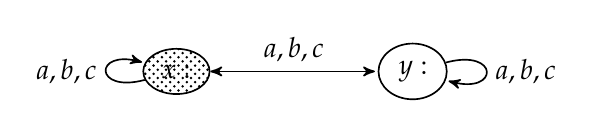
\begin{tikzpicture}[<->,>=stealth',shorten >=1pt,auto,node distance=4cm,semithick]
\tikzstyle{every ellipse node}= [draw]
\path (-1.5,0) node[ellipse,pattern = crosshatch dots]  (x) {$x: \heads $}  --
 (1.5,0) node[ellipse,draw](y)  {$y: \tails$} ;
%\path[<->] (x) edge  (y);
\draw (x) -- (y) node[midway,above] {$a,b,c$};
% \draw[<->]  (x) -- {a,b} (y);
\path[->] (x) edge [loop left]  node {$a,b,c$} (x);
\path[->] (y) edge [loop right] node {$a,b,c$} (y);
 \end{tikzpicture}
 $$

Suppose  that we consider a scenario 
where $A$ looks at the coin,
$B$ sees this (but not the result),
$C$ is distracted and
thinks nothing happened, and 
$A$ and $B$ are fully aware of each other and of $C$.
An action model $\Sigma$ for this is
$$
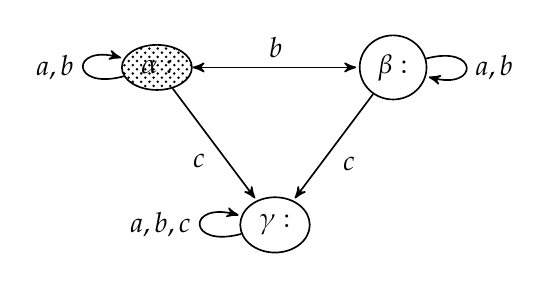
\begin{tikzpicture}[<->,>=stealth',shorten >=1pt,auto,node distance=4cm,semithick]
\tikzstyle{every ellipse node}= [draw]
\path (-1.5,1) node[ellipse,pattern = crosshatch dots]  (x) {$\alpha: \heads $}  --
 (1.5,1) node[ellipse,draw](y)  {$\beta: \tails$} ;
%\path[<->] (x) edge  (y);
\draw (x) -- (y) node[midway,above] {$b$};
% \draw[<->]  (x) -- {a,b} (y);
\path[->] (x) edge [loop left]  node {$a,b$} (x);
\path[->] (y) edge [loop right] node {$a,b$} (y);
\path (0,-1) node[ellipse]  (u) {$\gamma: \heads $};
%  --
 %(1.5,-1) node[ellipse,draw](v)  {$\delta: \tails$} ;
 \path[->] (u) edge [loop left]  node {$a,b,c$} (u);
%\path[->] (v) edge [loop right] node {$a,b,c$} (v);
%\draw (u) -- (v) node[midway,below] {$a,b,c$};
\path[->] (x) edge node [swap] {$c$} (u);
%\path[->] (x) edge node [near end] {$c$} (v);
\path[->] (y) edge node {$c$} (u);
%\path[->] (y) edge node {$c$} (v);
 \end{tikzpicture}
 $$
 Calculate $\Model\otimes \Sigma$.

\item   Now suppose that $C$ ``cheats'' and takes a look in
the ``completely private way'' that we model as a private announcement.
Write out the action model  $\Sigma'$
this time, and then compute the new model $(\Model\otimes \Sigma)\otimes \Sigma'$ by 
taking the action product.
(Part of the problem is to figure out what $\Sigma'$ should be.)

}

\item
Suppose we take the two muddy children, from class on November 18.
But now we want to change things so that $A$ is \emph{blind}: she can't see anything.
And let's assume that $B$ knows this.


\begin{enumerate}
\item  In the semantics, what happens when we run the muddy children scnenario with $A$ clean and $B$ muddy?
That is, we first announce that \emph{at least one of you is muddy}, and then the two of them announce whether they 
know or not; they announce this repeatedly.
\item  In the semantics, what happens when we run the muddy children scnenario with $A$ muddy and $B$ clean?
That is, we first announce that \emph{at least one of you is muddy}, and then the two of them announce whether they 
know or not; they announce this repeatedly.
\item
Now we want to do the previous two parts in the proof theory.  You should have two derivations, similar to what we did in 
class when both $A$ and $B$ were sighted.

\end{enumerate}



\end{enumerate}

\end{document}
